% Created by tikzDevice version 0.12.3.1 on 2021-11-25 03:30:16
% !TEX encoding = UTF-8 Unicode
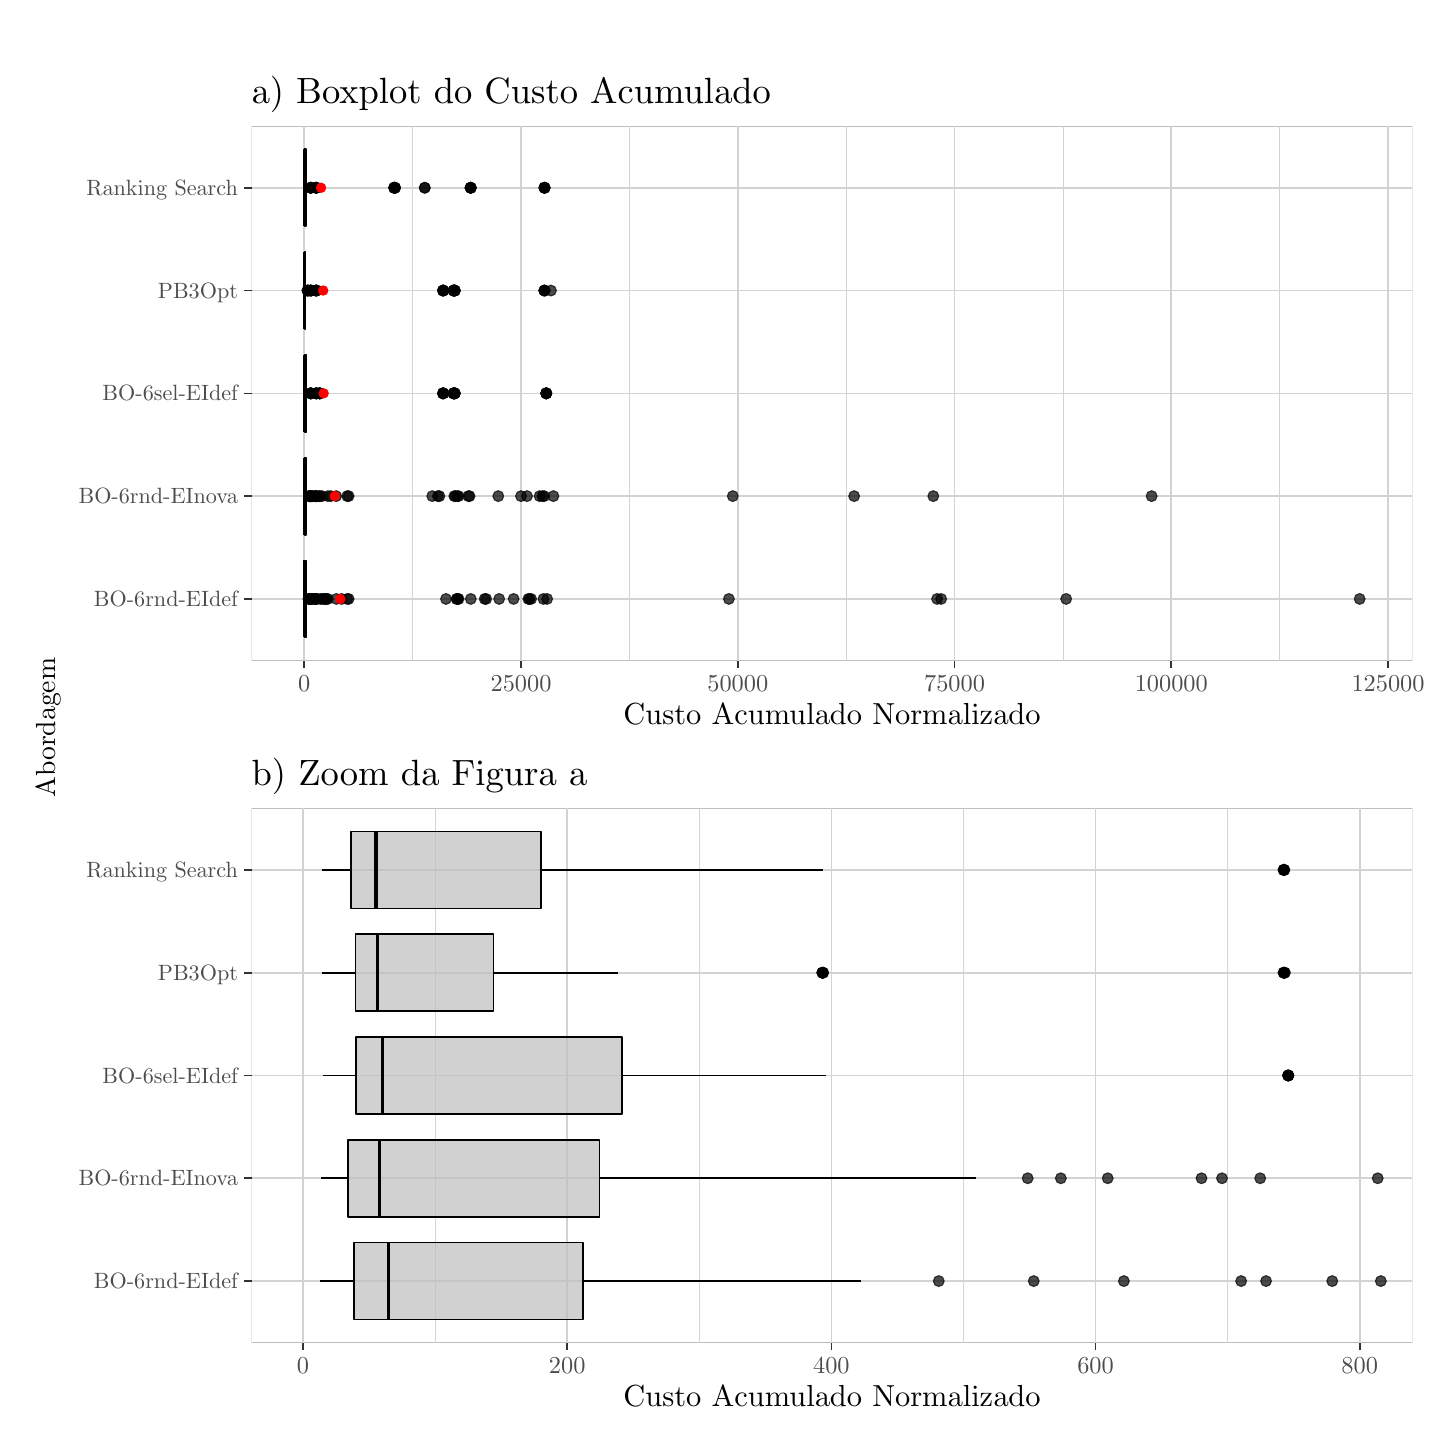
\begin{tikzpicture}[x=1pt,y=1pt]
\definecolor{fillColor}{RGB}{255,255,255}
\path[use as bounding box,fill=fillColor,fill opacity=0.00] (0,0) rectangle (505.89,505.89);
\begin{scope}
\path[clip] ( 12.91,246.49) rectangle (505.89,492.98);
\definecolor{drawColor}{RGB}{255,255,255}
\definecolor{fillColor}{RGB}{255,255,255}

\path[draw=drawColor,line width= 0.6pt,line join=round,line cap=round,fill=fillColor] ( 12.91,246.49) rectangle (505.89,492.98);
\end{scope}
\begin{scope}
\path[clip] ( 80.92,277.18) rectangle (500.39,470.32);
\definecolor{drawColor}{RGB}{190,190,190}
\definecolor{fillColor}{RGB}{255,255,255}

\path[draw=drawColor,line width= 0.6pt,line join=round,line cap=round,fill=fillColor] ( 80.92,277.18) rectangle (500.39,470.32);
\definecolor{drawColor}{RGB}{211,211,211}

\path[draw=drawColor,line width= 0.3pt,line join=round] (139.11,277.18) --
	(139.11,470.32);

\path[draw=drawColor,line width= 0.3pt,line join=round] (217.44,277.18) --
	(217.44,470.32);

\path[draw=drawColor,line width= 0.3pt,line join=round] (295.76,277.18) --
	(295.76,470.32);

\path[draw=drawColor,line width= 0.3pt,line join=round] (374.09,277.18) --
	(374.09,470.32);

\path[draw=drawColor,line width= 0.3pt,line join=round] (452.42,277.18) --
	(452.42,470.32);

\path[draw=drawColor,line width= 0.6pt,line join=round] ( 80.92,299.46) --
	(500.39,299.46);

\path[draw=drawColor,line width= 0.6pt,line join=round] ( 80.92,336.61) --
	(500.39,336.61);

\path[draw=drawColor,line width= 0.6pt,line join=round] ( 80.92,373.75) --
	(500.39,373.75);

\path[draw=drawColor,line width= 0.6pt,line join=round] ( 80.92,410.89) --
	(500.39,410.89);

\path[draw=drawColor,line width= 0.6pt,line join=round] ( 80.92,448.04) --
	(500.39,448.04);

\path[draw=drawColor,line width= 0.6pt,line join=round] ( 99.95,277.18) --
	( 99.95,470.32);

\path[draw=drawColor,line width= 0.6pt,line join=round] (178.27,277.18) --
	(178.27,470.32);

\path[draw=drawColor,line width= 0.6pt,line join=round] (256.60,277.18) --
	(256.60,470.32);

\path[draw=drawColor,line width= 0.6pt,line join=round] (334.93,277.18) --
	(334.93,470.32);

\path[draw=drawColor,line width= 0.6pt,line join=round] (413.25,277.18) --
	(413.25,470.32);

\path[draw=drawColor,line width= 0.6pt,line join=round] (491.58,277.18) --
	(491.58,470.32);
\definecolor{drawColor}{RGB}{0,0,0}
\definecolor{fillColor}{RGB}{0,0,0}

\path[draw=drawColor,draw opacity=0.70,line width= 0.4pt,line join=round,line cap=round,fill=fillColor,fill opacity=0.70] (330.08,299.46) circle (  1.96);

\path[draw=drawColor,draw opacity=0.70,line width= 0.4pt,line join=round,line cap=round,fill=fillColor,fill opacity=0.70] (115.46,299.46) circle (  1.96);

\path[draw=drawColor,draw opacity=0.70,line width= 0.4pt,line join=round,line cap=round,fill=fillColor,fill opacity=0.70] (105.70,299.46) circle (  1.96);

\path[draw=drawColor,draw opacity=0.70,line width= 0.4pt,line join=round,line cap=round,fill=fillColor,fill opacity=0.70] (107.41,299.46) circle (  1.96);

\path[draw=drawColor,draw opacity=0.70,line width= 0.4pt,line join=round,line cap=round,fill=fillColor,fill opacity=0.70] (103.87,299.46) circle (  1.96);

\path[draw=drawColor,draw opacity=0.70,line width= 0.4pt,line join=round,line cap=round,fill=fillColor,fill opacity=0.70] (181.92,299.46) circle (  1.96);

\path[draw=drawColor,draw opacity=0.70,line width= 0.4pt,line join=round,line cap=round,fill=fillColor,fill opacity=0.70] (154.96,299.46) circle (  1.96);

\path[draw=drawColor,draw opacity=0.70,line width= 0.4pt,line join=round,line cap=round,fill=fillColor,fill opacity=0.70] (180.91,299.46) circle (  1.96);

\path[draw=drawColor,draw opacity=0.70,line width= 0.4pt,line join=round,line cap=round,fill=fillColor,fill opacity=0.70] (375.25,299.46) circle (  1.96);

\path[draw=drawColor,draw opacity=0.70,line width= 0.4pt,line join=round,line cap=round,fill=fillColor,fill opacity=0.70] (107.80,299.46) circle (  1.96);

\path[draw=drawColor,draw opacity=0.70,line width= 0.4pt,line join=round,line cap=round,fill=fillColor,fill opacity=0.70] (102.39,299.46) circle (  1.96);

\path[draw=drawColor,draw opacity=0.70,line width= 0.4pt,line join=round,line cap=round,fill=fillColor,fill opacity=0.70] (104.24,299.46) circle (  1.96);

\path[draw=drawColor,draw opacity=0.70,line width= 0.4pt,line join=round,line cap=round,fill=fillColor,fill opacity=0.70] (155.44,299.46) circle (  1.96);

\path[draw=drawColor,draw opacity=0.70,line width= 0.4pt,line join=round,line cap=round,fill=fillColor,fill opacity=0.70] (165.15,299.46) circle (  1.96);

\path[draw=drawColor,draw opacity=0.70,line width= 0.4pt,line join=round,line cap=round,fill=fillColor,fill opacity=0.70] (175.60,299.46) circle (  1.96);

\path[draw=drawColor,draw opacity=0.70,line width= 0.4pt,line join=round,line cap=round,fill=fillColor,fill opacity=0.70] (253.38,299.46) circle (  1.96);

\path[draw=drawColor,draw opacity=0.70,line width= 0.4pt,line join=round,line cap=round,fill=fillColor,fill opacity=0.70] (113.42,299.46) circle (  1.96);

\path[draw=drawColor,draw opacity=0.70,line width= 0.4pt,line join=round,line cap=round,fill=fillColor,fill opacity=0.70] (102.70,299.46) circle (  1.96);

\path[draw=drawColor,draw opacity=0.70,line width= 0.4pt,line join=round,line cap=round,fill=fillColor,fill opacity=0.70] (108.49,299.46) circle (  1.96);

\path[draw=drawColor,draw opacity=0.70,line width= 0.4pt,line join=round,line cap=round,fill=fillColor,fill opacity=0.70] (102.51,299.46) circle (  1.96);

\path[draw=drawColor,draw opacity=0.70,line width= 0.4pt,line join=round,line cap=round,fill=fillColor,fill opacity=0.70] (104.45,299.46) circle (  1.96);

\path[draw=drawColor,draw opacity=0.70,line width= 0.4pt,line join=round,line cap=round,fill=fillColor,fill opacity=0.70] (155.70,299.46) circle (  1.96);

\path[draw=drawColor,draw opacity=0.70,line width= 0.4pt,line join=round,line cap=round,fill=fillColor,fill opacity=0.70] (155.25,299.46) circle (  1.96);

\path[draw=drawColor,draw opacity=0.70,line width= 0.4pt,line join=round,line cap=round,fill=fillColor,fill opacity=0.70] (151.16,299.46) circle (  1.96);

\path[draw=drawColor,draw opacity=0.70,line width= 0.4pt,line join=round,line cap=round,fill=fillColor,fill opacity=0.70] (101.68,299.46) circle (  1.96);

\path[draw=drawColor,draw opacity=0.70,line width= 0.4pt,line join=round,line cap=round,fill=fillColor,fill opacity=0.70] (481.32,299.46) circle (  1.96);

\path[draw=drawColor,draw opacity=0.70,line width= 0.4pt,line join=round,line cap=round,fill=fillColor,fill opacity=0.70] (111.55,299.46) circle (  1.96);

\path[draw=drawColor,draw opacity=0.70,line width= 0.4pt,line join=round,line cap=round,fill=fillColor,fill opacity=0.70] (115.98,299.46) circle (  1.96);

\path[draw=drawColor,draw opacity=0.70,line width= 0.4pt,line join=round,line cap=round,fill=fillColor,fill opacity=0.70] (104.26,299.46) circle (  1.96);

\path[draw=drawColor,draw opacity=0.70,line width= 0.4pt,line join=round,line cap=round,fill=fillColor,fill opacity=0.70] (102.17,299.46) circle (  1.96);

\path[draw=drawColor,draw opacity=0.70,line width= 0.4pt,line join=round,line cap=round,fill=fillColor,fill opacity=0.70] (102.23,299.46) circle (  1.96);

\path[draw=drawColor,draw opacity=0.70,line width= 0.4pt,line join=round,line cap=round,fill=fillColor,fill opacity=0.70] (187.70,299.46) circle (  1.96);

\path[draw=drawColor,draw opacity=0.70,line width= 0.4pt,line join=round,line cap=round,fill=fillColor,fill opacity=0.70] (181.30,299.46) circle (  1.96);

\path[draw=drawColor,draw opacity=0.70,line width= 0.4pt,line join=round,line cap=round,fill=fillColor,fill opacity=0.70] (170.37,299.46) circle (  1.96);

\path[draw=drawColor,draw opacity=0.70,line width= 0.4pt,line join=round,line cap=round,fill=fillColor,fill opacity=0.70] (328.61,299.46) circle (  1.96);

\path[draw=drawColor,draw opacity=0.70,line width= 0.4pt,line join=round,line cap=round,fill=fillColor,fill opacity=0.70] (107.76,299.46) circle (  1.96);

\path[draw=drawColor,draw opacity=0.70,line width= 0.4pt,line join=round,line cap=round,fill=fillColor,fill opacity=0.70] (107.05,299.46) circle (  1.96);

\path[draw=drawColor,draw opacity=0.70,line width= 0.4pt,line join=round,line cap=round,fill=fillColor,fill opacity=0.70] (101.46,299.46) circle (  1.96);

\path[draw=drawColor,draw opacity=0.70,line width= 0.4pt,line join=round,line cap=round,fill=fillColor,fill opacity=0.70] (106.37,299.46) circle (  1.96);

\path[draw=drawColor,draw opacity=0.70,line width= 0.4pt,line join=round,line cap=round,fill=fillColor,fill opacity=0.70] (101.90,299.46) circle (  1.96);

\path[draw=drawColor,draw opacity=0.70,line width= 0.4pt,line join=round,line cap=round,fill=fillColor,fill opacity=0.70] (103.33,299.46) circle (  1.96);

\path[draw=drawColor,draw opacity=0.70,line width= 0.4pt,line join=round,line cap=round,fill=fillColor,fill opacity=0.70] (165.68,299.46) circle (  1.96);

\path[draw=drawColor,draw opacity=0.70,line width= 0.4pt,line join=round,line cap=round,fill=fillColor,fill opacity=0.70] (186.37,299.46) circle (  1.96);

\path[draw=drawColor,draw opacity=0.70,line width= 0.4pt,line join=round,line cap=round,fill=fillColor,fill opacity=0.70] (160.12,299.46) circle (  1.96);
\definecolor{drawColor}{RGB}{0,0,0}

\path[draw=drawColor,line width= 0.6pt,line join=round] (100.61,299.46) -- (101.27,299.46);

\path[draw=drawColor,line width= 0.6pt,line join=round] (100.07,299.46) -- ( 99.99,299.46);
\definecolor{fillColor}{RGB}{190,190,190}

\path[draw=drawColor,line width= 0.6pt,line join=round,line cap=round,fill=fillColor,fill opacity=0.70] (100.61,285.53) --
	(100.07,285.53) --
	(100.07,313.39) --
	(100.61,313.39) --
	(100.61,285.53) --
	cycle;

\path[draw=drawColor,line width= 1.1pt,line join=round] (100.15,285.53) -- (100.15,313.39);
\definecolor{drawColor}{RGB}{0,0,0}
\definecolor{fillColor}{RGB}{0,0,0}

\path[draw=drawColor,draw opacity=0.70,line width= 0.4pt,line join=round,line cap=round,fill=fillColor,fill opacity=0.70] (254.79,336.61) circle (  1.96);

\path[draw=drawColor,draw opacity=0.70,line width= 0.4pt,line join=round,line cap=round,fill=fillColor,fill opacity=0.70] (115.47,336.61) circle (  1.96);

\path[draw=drawColor,draw opacity=0.70,line width= 0.4pt,line join=round,line cap=round,fill=fillColor,fill opacity=0.70] (105.60,336.61) circle (  1.96);

\path[draw=drawColor,draw opacity=0.70,line width= 0.4pt,line join=round,line cap=round,fill=fillColor,fill opacity=0.70] (105.28,336.61) circle (  1.96);

\path[draw=drawColor,draw opacity=0.70,line width= 0.4pt,line join=round,line cap=round,fill=fillColor,fill opacity=0.70] (102.76,336.61) circle (  1.96);

\path[draw=drawColor,draw opacity=0.70,line width= 0.4pt,line join=round,line cap=round,fill=fillColor,fill opacity=0.70] (159.68,336.61) circle (  1.96);

\path[draw=drawColor,draw opacity=0.70,line width= 0.4pt,line join=round,line cap=round,fill=fillColor,fill opacity=0.70] (148.20,336.61) circle (  1.96);

\path[draw=drawColor,draw opacity=0.70,line width= 0.4pt,line join=round,line cap=round,fill=fillColor,fill opacity=0.70] (180.43,336.61) circle (  1.96);

\path[draw=drawColor,draw opacity=0.70,line width= 0.4pt,line join=round,line cap=round,fill=fillColor,fill opacity=0.70] (298.64,336.61) circle (  1.96);

\path[draw=drawColor,draw opacity=0.70,line width= 0.4pt,line join=round,line cap=round,fill=fillColor,fill opacity=0.70] (104.01,336.61) circle (  1.96);

\path[draw=drawColor,draw opacity=0.70,line width= 0.4pt,line join=round,line cap=round,fill=fillColor,fill opacity=0.70] (102.08,336.61) circle (  1.96);

\path[draw=drawColor,draw opacity=0.70,line width= 0.4pt,line join=round,line cap=round,fill=fillColor,fill opacity=0.70] (102.13,336.61) circle (  1.96);

\path[draw=drawColor,draw opacity=0.70,line width= 0.4pt,line join=round,line cap=round,fill=fillColor,fill opacity=0.70] (148.79,336.61) circle (  1.96);

\path[draw=drawColor,draw opacity=0.70,line width= 0.4pt,line join=round,line cap=round,fill=fillColor,fill opacity=0.70] (154.15,336.61) circle (  1.96);

\path[draw=drawColor,draw opacity=0.70,line width= 0.4pt,line join=round,line cap=round,fill=fillColor,fill opacity=0.70] (184.97,336.61) circle (  1.96);

\path[draw=drawColor,draw opacity=0.70,line width= 0.4pt,line join=round,line cap=round,fill=fillColor,fill opacity=0.70] (178.26,336.61) circle (  1.96);

\path[draw=drawColor,draw opacity=0.70,line width= 0.4pt,line join=round,line cap=round,fill=fillColor,fill opacity=0.70] (109.57,336.61) circle (  1.96);

\path[draw=drawColor,draw opacity=0.70,line width= 0.4pt,line join=round,line cap=round,fill=fillColor,fill opacity=0.70] (108.49,336.61) circle (  1.96);

\path[draw=drawColor,draw opacity=0.70,line width= 0.4pt,line join=round,line cap=round,fill=fillColor,fill opacity=0.70] (102.50,336.61) circle (  1.96);

\path[draw=drawColor,draw opacity=0.70,line width= 0.4pt,line join=round,line cap=round,fill=fillColor,fill opacity=0.70] (104.44,336.61) circle (  1.96);

\path[draw=drawColor,draw opacity=0.70,line width= 0.4pt,line join=round,line cap=round,fill=fillColor,fill opacity=0.70] (155.70,336.61) circle (  1.96);

\path[draw=drawColor,draw opacity=0.70,line width= 0.4pt,line join=round,line cap=round,fill=fillColor,fill opacity=0.70] (155.25,336.61) circle (  1.96);

\path[draw=drawColor,draw opacity=0.70,line width= 0.4pt,line join=round,line cap=round,fill=fillColor,fill opacity=0.70] (146.18,336.61) circle (  1.96);

\path[draw=drawColor,draw opacity=0.70,line width= 0.4pt,line join=round,line cap=round,fill=fillColor,fill opacity=0.70] (101.67,336.61) circle (  1.96);

\path[draw=drawColor,draw opacity=0.70,line width= 0.4pt,line join=round,line cap=round,fill=fillColor,fill opacity=0.70] (406.14,336.61) circle (  1.96);

\path[draw=drawColor,draw opacity=0.70,line width= 0.4pt,line join=round,line cap=round,fill=fillColor,fill opacity=0.70] (111.48,336.61) circle (  1.96);

\path[draw=drawColor,draw opacity=0.70,line width= 0.4pt,line join=round,line cap=round,fill=fillColor,fill opacity=0.70] (115.98,336.61) circle (  1.96);

\path[draw=drawColor,draw opacity=0.70,line width= 0.4pt,line join=round,line cap=round,fill=fillColor,fill opacity=0.70] (104.24,336.61) circle (  1.96);

\path[draw=drawColor,draw opacity=0.70,line width= 0.4pt,line join=round,line cap=round,fill=fillColor,fill opacity=0.70] (102.22,336.61) circle (  1.96);

\path[draw=drawColor,draw opacity=0.70,line width= 0.4pt,line join=round,line cap=round,fill=fillColor,fill opacity=0.70] (186.65,336.61) circle (  1.96);

\path[draw=drawColor,draw opacity=0.70,line width= 0.4pt,line join=round,line cap=round,fill=fillColor,fill opacity=0.70] (159.24,336.61) circle (  1.96);

\path[draw=drawColor,draw opacity=0.70,line width= 0.4pt,line join=round,line cap=round,fill=fillColor,fill opacity=0.70] (189.97,336.61) circle (  1.96);

\path[draw=drawColor,draw opacity=0.70,line width= 0.4pt,line join=round,line cap=round,fill=fillColor,fill opacity=0.70] (327.24,336.61) circle (  1.96);

\path[draw=drawColor,draw opacity=0.70,line width= 0.4pt,line join=round,line cap=round,fill=fillColor,fill opacity=0.70] (103.91,336.61) circle (  1.96);

\path[draw=drawColor,draw opacity=0.70,line width= 0.4pt,line join=round,line cap=round,fill=fillColor,fill opacity=0.70] (101.75,336.61) circle (  1.96);

\path[draw=drawColor,draw opacity=0.70,line width= 0.4pt,line join=round,line cap=round,fill=fillColor,fill opacity=0.70] (106.34,336.61) circle (  1.96);

\path[draw=drawColor,draw opacity=0.70,line width= 0.4pt,line join=round,line cap=round,fill=fillColor,fill opacity=0.70] (101.86,336.61) circle (  1.96);

\path[draw=drawColor,draw opacity=0.70,line width= 0.4pt,line join=round,line cap=round,fill=fillColor,fill opacity=0.70] (103.32,336.61) circle (  1.96);

\path[draw=drawColor,draw opacity=0.70,line width= 0.4pt,line join=round,line cap=round,fill=fillColor,fill opacity=0.70] (154.58,336.61) circle (  1.96);

\path[draw=drawColor,draw opacity=0.70,line width= 0.4pt,line join=round,line cap=round,fill=fillColor,fill opacity=0.70] (186.02,336.61) circle (  1.96);

\path[draw=drawColor,draw opacity=0.70,line width= 0.4pt,line join=round,line cap=round,fill=fillColor,fill opacity=0.70] (170.05,336.61) circle (  1.96);
\definecolor{drawColor}{RGB}{0,0,0}

\path[draw=drawColor,line width= 0.6pt,line join=round] (100.65,336.61) -- (101.55,336.61);

\path[draw=drawColor,line width= 0.6pt,line join=round] (100.06,336.61) -- ( 99.99,336.61);
\definecolor{fillColor}{RGB}{190,190,190}

\path[draw=drawColor,line width= 0.6pt,line join=round,line cap=round,fill=fillColor,fill opacity=0.70] (100.65,322.68) --
	(100.06,322.68) --
	(100.06,350.53) --
	(100.65,350.53) --
	(100.65,322.68) --
	cycle;

\path[draw=drawColor,line width= 1.1pt,line join=round] (100.13,322.68) -- (100.13,350.53);
\definecolor{drawColor}{RGB}{0,0,0}
\definecolor{fillColor}{RGB}{0,0,0}

\path[draw=drawColor,draw opacity=0.70,line width= 0.4pt,line join=round,line cap=round,fill=fillColor,fill opacity=0.70] (187.39,373.75) circle (  1.96);

\path[draw=drawColor,draw opacity=0.70,line width= 0.4pt,line join=round,line cap=round,fill=fillColor,fill opacity=0.70] (104.31,373.75) circle (  1.96);

\path[draw=drawColor,draw opacity=0.70,line width= 0.4pt,line join=round,line cap=round,fill=fillColor,fill opacity=0.70] (105.53,373.75) circle (  1.96);

\path[draw=drawColor,draw opacity=0.70,line width= 0.4pt,line join=round,line cap=round,fill=fillColor,fill opacity=0.70] (102.29,373.75) circle (  1.96);

\path[draw=drawColor,draw opacity=0.70,line width= 0.4pt,line join=round,line cap=round,fill=fillColor,fill opacity=0.70] (154.29,373.75) circle (  1.96);

\path[draw=drawColor,draw opacity=0.70,line width= 0.4pt,line join=round,line cap=round,fill=fillColor,fill opacity=0.70] (153.89,373.75) circle (  1.96);

\path[draw=drawColor,draw opacity=0.70,line width= 0.4pt,line join=round,line cap=round,fill=fillColor,fill opacity=0.70] (150.12,373.75) circle (  1.96);

\path[draw=drawColor,draw opacity=0.70,line width= 0.4pt,line join=round,line cap=round,fill=fillColor,fill opacity=0.70] (187.39,373.75) circle (  1.96);

\path[draw=drawColor,draw opacity=0.70,line width= 0.4pt,line join=round,line cap=round,fill=fillColor,fill opacity=0.70] (104.31,373.75) circle (  1.96);

\path[draw=drawColor,draw opacity=0.70,line width= 0.4pt,line join=round,line cap=round,fill=fillColor,fill opacity=0.70] (105.53,373.75) circle (  1.96);

\path[draw=drawColor,draw opacity=0.70,line width= 0.4pt,line join=round,line cap=round,fill=fillColor,fill opacity=0.70] (102.29,373.75) circle (  1.96);

\path[draw=drawColor,draw opacity=0.70,line width= 0.4pt,line join=round,line cap=round,fill=fillColor,fill opacity=0.70] (154.29,373.75) circle (  1.96);

\path[draw=drawColor,draw opacity=0.70,line width= 0.4pt,line join=round,line cap=round,fill=fillColor,fill opacity=0.70] (153.89,373.75) circle (  1.96);

\path[draw=drawColor,draw opacity=0.70,line width= 0.4pt,line join=round,line cap=round,fill=fillColor,fill opacity=0.70] (150.12,373.75) circle (  1.96);

\path[draw=drawColor,draw opacity=0.70,line width= 0.4pt,line join=round,line cap=round,fill=fillColor,fill opacity=0.70] (187.39,373.75) circle (  1.96);

\path[draw=drawColor,draw opacity=0.70,line width= 0.4pt,line join=round,line cap=round,fill=fillColor,fill opacity=0.70] (104.31,373.75) circle (  1.96);

\path[draw=drawColor,draw opacity=0.70,line width= 0.4pt,line join=round,line cap=round,fill=fillColor,fill opacity=0.70] (105.53,373.75) circle (  1.96);

\path[draw=drawColor,draw opacity=0.70,line width= 0.4pt,line join=round,line cap=round,fill=fillColor,fill opacity=0.70] (102.29,373.75) circle (  1.96);

\path[draw=drawColor,draw opacity=0.70,line width= 0.4pt,line join=round,line cap=round,fill=fillColor,fill opacity=0.70] (154.29,373.75) circle (  1.96);

\path[draw=drawColor,draw opacity=0.70,line width= 0.4pt,line join=round,line cap=round,fill=fillColor,fill opacity=0.70] (153.89,373.75) circle (  1.96);

\path[draw=drawColor,draw opacity=0.70,line width= 0.4pt,line join=round,line cap=round,fill=fillColor,fill opacity=0.70] (150.12,373.75) circle (  1.96);

\path[draw=drawColor,draw opacity=0.70,line width= 0.4pt,line join=round,line cap=round,fill=fillColor,fill opacity=0.70] (187.39,373.75) circle (  1.96);

\path[draw=drawColor,draw opacity=0.70,line width= 0.4pt,line join=round,line cap=round,fill=fillColor,fill opacity=0.70] (104.31,373.75) circle (  1.96);

\path[draw=drawColor,draw opacity=0.70,line width= 0.4pt,line join=round,line cap=round,fill=fillColor,fill opacity=0.70] (105.53,373.75) circle (  1.96);

\path[draw=drawColor,draw opacity=0.70,line width= 0.4pt,line join=round,line cap=round,fill=fillColor,fill opacity=0.70] (102.29,373.75) circle (  1.96);

\path[draw=drawColor,draw opacity=0.70,line width= 0.4pt,line join=round,line cap=round,fill=fillColor,fill opacity=0.70] (154.29,373.75) circle (  1.96);

\path[draw=drawColor,draw opacity=0.70,line width= 0.4pt,line join=round,line cap=round,fill=fillColor,fill opacity=0.70] (153.89,373.75) circle (  1.96);

\path[draw=drawColor,draw opacity=0.70,line width= 0.4pt,line join=round,line cap=round,fill=fillColor,fill opacity=0.70] (150.12,373.75) circle (  1.96);

\path[draw=drawColor,draw opacity=0.70,line width= 0.4pt,line join=round,line cap=round,fill=fillColor,fill opacity=0.70] (187.39,373.75) circle (  1.96);

\path[draw=drawColor,draw opacity=0.70,line width= 0.4pt,line join=round,line cap=round,fill=fillColor,fill opacity=0.70] (104.31,373.75) circle (  1.96);

\path[draw=drawColor,draw opacity=0.70,line width= 0.4pt,line join=round,line cap=round,fill=fillColor,fill opacity=0.70] (105.53,373.75) circle (  1.96);

\path[draw=drawColor,draw opacity=0.70,line width= 0.4pt,line join=round,line cap=round,fill=fillColor,fill opacity=0.70] (102.29,373.75) circle (  1.96);

\path[draw=drawColor,draw opacity=0.70,line width= 0.4pt,line join=round,line cap=round,fill=fillColor,fill opacity=0.70] (154.29,373.75) circle (  1.96);

\path[draw=drawColor,draw opacity=0.70,line width= 0.4pt,line join=round,line cap=round,fill=fillColor,fill opacity=0.70] (153.89,373.75) circle (  1.96);

\path[draw=drawColor,draw opacity=0.70,line width= 0.4pt,line join=round,line cap=round,fill=fillColor,fill opacity=0.70] (150.12,373.75) circle (  1.96);
\definecolor{drawColor}{RGB}{0,0,0}

\path[draw=drawColor,line width= 0.6pt,line join=round] (100.71,373.75) -- (101.19,373.75);

\path[draw=drawColor,line width= 0.6pt,line join=round] (100.07,373.75) -- (100.00,373.75);
\definecolor{fillColor}{RGB}{190,190,190}

\path[draw=drawColor,line width= 0.6pt,line join=round,line cap=round,fill=fillColor,fill opacity=0.70] (100.71,359.82) --
	(100.07,359.82) --
	(100.07,387.68) --
	(100.71,387.68) --
	(100.71,359.82) --
	cycle;

\path[draw=drawColor,line width= 1.1pt,line join=round] (100.14,359.82) -- (100.14,387.68);
\definecolor{drawColor}{RGB}{0,0,0}
\definecolor{fillColor}{RGB}{0,0,0}

\path[draw=drawColor,draw opacity=0.70,line width= 0.4pt,line join=round,line cap=round,fill=fillColor,fill opacity=0.70] (186.71,410.89) circle (  1.96);

\path[draw=drawColor,draw opacity=0.70,line width= 0.4pt,line join=round,line cap=round,fill=fillColor,fill opacity=0.70] (104.27,410.89) circle (  1.96);

\path[draw=drawColor,draw opacity=0.70,line width= 0.4pt,line join=round,line cap=round,fill=fillColor,fill opacity=0.70] (102.28,410.89) circle (  1.96);

\path[draw=drawColor,draw opacity=0.70,line width= 0.4pt,line join=round,line cap=round,fill=fillColor,fill opacity=0.70] (101.18,410.89) circle (  1.96);

\path[draw=drawColor,draw opacity=0.70,line width= 0.4pt,line join=round,line cap=round,fill=fillColor,fill opacity=0.70] (154.30,410.89) circle (  1.96);

\path[draw=drawColor,draw opacity=0.70,line width= 0.4pt,line join=round,line cap=round,fill=fillColor,fill opacity=0.70] (153.90,410.89) circle (  1.96);

\path[draw=drawColor,draw opacity=0.70,line width= 0.4pt,line join=round,line cap=round,fill=fillColor,fill opacity=0.70] (150.13,410.89) circle (  1.96);

\path[draw=drawColor,draw opacity=0.70,line width= 0.4pt,line join=round,line cap=round,fill=fillColor,fill opacity=0.70] (186.71,410.89) circle (  1.96);

\path[draw=drawColor,draw opacity=0.70,line width= 0.4pt,line join=round,line cap=round,fill=fillColor,fill opacity=0.70] (104.27,410.89) circle (  1.96);

\path[draw=drawColor,draw opacity=0.70,line width= 0.4pt,line join=round,line cap=round,fill=fillColor,fill opacity=0.70] (102.27,410.89) circle (  1.96);

\path[draw=drawColor,draw opacity=0.70,line width= 0.4pt,line join=round,line cap=round,fill=fillColor,fill opacity=0.70] (101.18,410.89) circle (  1.96);

\path[draw=drawColor,draw opacity=0.70,line width= 0.4pt,line join=round,line cap=round,fill=fillColor,fill opacity=0.70] (154.30,410.89) circle (  1.96);

\path[draw=drawColor,draw opacity=0.70,line width= 0.4pt,line join=round,line cap=round,fill=fillColor,fill opacity=0.70] (153.90,410.89) circle (  1.96);

\path[draw=drawColor,draw opacity=0.70,line width= 0.4pt,line join=round,line cap=round,fill=fillColor,fill opacity=0.70] (150.13,410.89) circle (  1.96);

\path[draw=drawColor,draw opacity=0.70,line width= 0.4pt,line join=round,line cap=round,fill=fillColor,fill opacity=0.70] (189.08,410.89) circle (  1.96);

\path[draw=drawColor,draw opacity=0.70,line width= 0.4pt,line join=round,line cap=round,fill=fillColor,fill opacity=0.70] (104.30,410.89) circle (  1.96);

\path[draw=drawColor,draw opacity=0.70,line width= 0.4pt,line join=round,line cap=round,fill=fillColor,fill opacity=0.70] (102.27,410.89) circle (  1.96);

\path[draw=drawColor,draw opacity=0.70,line width= 0.4pt,line join=round,line cap=round,fill=fillColor,fill opacity=0.70] (101.18,410.89) circle (  1.96);

\path[draw=drawColor,draw opacity=0.70,line width= 0.4pt,line join=round,line cap=round,fill=fillColor,fill opacity=0.70] (154.30,410.89) circle (  1.96);

\path[draw=drawColor,draw opacity=0.70,line width= 0.4pt,line join=round,line cap=round,fill=fillColor,fill opacity=0.70] (153.90,410.89) circle (  1.96);

\path[draw=drawColor,draw opacity=0.70,line width= 0.4pt,line join=round,line cap=round,fill=fillColor,fill opacity=0.70] (150.13,410.89) circle (  1.96);

\path[draw=drawColor,draw opacity=0.70,line width= 0.4pt,line join=round,line cap=round,fill=fillColor,fill opacity=0.70] (186.78,410.89) circle (  1.96);

\path[draw=drawColor,draw opacity=0.70,line width= 0.4pt,line join=round,line cap=round,fill=fillColor,fill opacity=0.70] (104.27,410.89) circle (  1.96);

\path[draw=drawColor,draw opacity=0.70,line width= 0.4pt,line join=round,line cap=round,fill=fillColor,fill opacity=0.70] (102.28,410.89) circle (  1.96);

\path[draw=drawColor,draw opacity=0.70,line width= 0.4pt,line join=round,line cap=round,fill=fillColor,fill opacity=0.70] (101.18,410.89) circle (  1.96);

\path[draw=drawColor,draw opacity=0.70,line width= 0.4pt,line join=round,line cap=round,fill=fillColor,fill opacity=0.70] (154.30,410.89) circle (  1.96);

\path[draw=drawColor,draw opacity=0.70,line width= 0.4pt,line join=round,line cap=round,fill=fillColor,fill opacity=0.70] (153.90,410.89) circle (  1.96);

\path[draw=drawColor,draw opacity=0.70,line width= 0.4pt,line join=round,line cap=round,fill=fillColor,fill opacity=0.70] (150.13,410.89) circle (  1.96);

\path[draw=drawColor,draw opacity=0.70,line width= 0.4pt,line join=round,line cap=round,fill=fillColor,fill opacity=0.70] (186.71,410.89) circle (  1.96);

\path[draw=drawColor,draw opacity=0.70,line width= 0.4pt,line join=round,line cap=round,fill=fillColor,fill opacity=0.70] (104.27,410.89) circle (  1.96);

\path[draw=drawColor,draw opacity=0.70,line width= 0.4pt,line join=round,line cap=round,fill=fillColor,fill opacity=0.70] (102.28,410.89) circle (  1.96);

\path[draw=drawColor,draw opacity=0.70,line width= 0.4pt,line join=round,line cap=round,fill=fillColor,fill opacity=0.70] (101.18,410.89) circle (  1.96);

\path[draw=drawColor,draw opacity=0.70,line width= 0.4pt,line join=round,line cap=round,fill=fillColor,fill opacity=0.70] (154.30,410.89) circle (  1.96);

\path[draw=drawColor,draw opacity=0.70,line width= 0.4pt,line join=round,line cap=round,fill=fillColor,fill opacity=0.70] (153.90,410.89) circle (  1.96);

\path[draw=drawColor,draw opacity=0.70,line width= 0.4pt,line join=round,line cap=round,fill=fillColor,fill opacity=0.70] (150.13,410.89) circle (  1.96);
\definecolor{drawColor}{RGB}{0,0,0}

\path[draw=drawColor,line width= 0.6pt,line join=round] (100.40,410.89) -- (100.70,410.89);

\path[draw=drawColor,line width= 0.6pt,line join=round] (100.07,410.89) -- ( 99.99,410.89);
\definecolor{fillColor}{RGB}{190,190,190}

\path[draw=drawColor,line width= 0.6pt,line join=round,line cap=round,fill=fillColor,fill opacity=0.70] (100.40,396.96) --
	(100.07,396.96) --
	(100.07,424.82) --
	(100.40,424.82) --
	(100.40,396.96) --
	cycle;

\path[draw=drawColor,line width= 1.1pt,line join=round] (100.13,396.96) -- (100.13,424.82);
\definecolor{drawColor}{RGB}{0,0,0}
\definecolor{fillColor}{RGB}{0,0,0}

\path[draw=drawColor,draw opacity=0.70,line width= 0.4pt,line join=round,line cap=round,fill=fillColor,fill opacity=0.70] (186.74,448.04) circle (  1.96);

\path[draw=drawColor,draw opacity=0.70,line width= 0.4pt,line join=round,line cap=round,fill=fillColor,fill opacity=0.70] (104.27,448.04) circle (  1.96);

\path[draw=drawColor,draw opacity=0.70,line width= 0.4pt,line join=round,line cap=round,fill=fillColor,fill opacity=0.70] (102.27,448.04) circle (  1.96);

\path[draw=drawColor,draw opacity=0.70,line width= 0.4pt,line join=round,line cap=round,fill=fillColor,fill opacity=0.70] (132.73,448.04) circle (  1.96);

\path[draw=drawColor,draw opacity=0.70,line width= 0.4pt,line join=round,line cap=round,fill=fillColor,fill opacity=0.70] (132.48,448.04) circle (  1.96);

\path[draw=drawColor,draw opacity=0.70,line width= 0.4pt,line join=round,line cap=round,fill=fillColor,fill opacity=0.70] (160.07,448.04) circle (  1.96);

\path[draw=drawColor,draw opacity=0.70,line width= 0.4pt,line join=round,line cap=round,fill=fillColor,fill opacity=0.70] (186.74,448.04) circle (  1.96);

\path[draw=drawColor,draw opacity=0.70,line width= 0.4pt,line join=round,line cap=round,fill=fillColor,fill opacity=0.70] (104.27,448.04) circle (  1.96);

\path[draw=drawColor,draw opacity=0.70,line width= 0.4pt,line join=round,line cap=round,fill=fillColor,fill opacity=0.70] (102.28,448.04) circle (  1.96);

\path[draw=drawColor,draw opacity=0.70,line width= 0.4pt,line join=round,line cap=round,fill=fillColor,fill opacity=0.70] (132.73,448.04) circle (  1.96);

\path[draw=drawColor,draw opacity=0.70,line width= 0.4pt,line join=round,line cap=round,fill=fillColor,fill opacity=0.70] (132.48,448.04) circle (  1.96);

\path[draw=drawColor,draw opacity=0.70,line width= 0.4pt,line join=round,line cap=round,fill=fillColor,fill opacity=0.70] (160.07,448.04) circle (  1.96);

\path[draw=drawColor,draw opacity=0.70,line width= 0.4pt,line join=round,line cap=round,fill=fillColor,fill opacity=0.70] (186.78,448.04) circle (  1.96);

\path[draw=drawColor,draw opacity=0.70,line width= 0.4pt,line join=round,line cap=round,fill=fillColor,fill opacity=0.70] (104.27,448.04) circle (  1.96);

\path[draw=drawColor,draw opacity=0.70,line width= 0.4pt,line join=round,line cap=round,fill=fillColor,fill opacity=0.70] (102.28,448.04) circle (  1.96);

\path[draw=drawColor,draw opacity=0.70,line width= 0.4pt,line join=round,line cap=round,fill=fillColor,fill opacity=0.70] (143.48,448.04) circle (  1.96);

\path[draw=drawColor,draw opacity=0.70,line width= 0.4pt,line join=round,line cap=round,fill=fillColor,fill opacity=0.70] (132.48,448.04) circle (  1.96);

\path[draw=drawColor,draw opacity=0.70,line width= 0.4pt,line join=round,line cap=round,fill=fillColor,fill opacity=0.70] (160.07,448.04) circle (  1.96);

\path[draw=drawColor,draw opacity=0.70,line width= 0.4pt,line join=round,line cap=round,fill=fillColor,fill opacity=0.70] (186.78,448.04) circle (  1.96);

\path[draw=drawColor,draw opacity=0.70,line width= 0.4pt,line join=round,line cap=round,fill=fillColor,fill opacity=0.70] (104.27,448.04) circle (  1.96);

\path[draw=drawColor,draw opacity=0.70,line width= 0.4pt,line join=round,line cap=round,fill=fillColor,fill opacity=0.70] (102.28,448.04) circle (  1.96);

\path[draw=drawColor,draw opacity=0.70,line width= 0.4pt,line join=round,line cap=round,fill=fillColor,fill opacity=0.70] (143.48,448.04) circle (  1.96);

\path[draw=drawColor,draw opacity=0.70,line width= 0.4pt,line join=round,line cap=round,fill=fillColor,fill opacity=0.70] (132.48,448.04) circle (  1.96);

\path[draw=drawColor,draw opacity=0.70,line width= 0.4pt,line join=round,line cap=round,fill=fillColor,fill opacity=0.70] (160.07,448.04) circle (  1.96);

\path[draw=drawColor,draw opacity=0.70,line width= 0.4pt,line join=round,line cap=round,fill=fillColor,fill opacity=0.70] (186.74,448.04) circle (  1.96);

\path[draw=drawColor,draw opacity=0.70,line width= 0.4pt,line join=round,line cap=round,fill=fillColor,fill opacity=0.70] (104.27,448.04) circle (  1.96);

\path[draw=drawColor,draw opacity=0.70,line width= 0.4pt,line join=round,line cap=round,fill=fillColor,fill opacity=0.70] (102.28,448.04) circle (  1.96);

\path[draw=drawColor,draw opacity=0.70,line width= 0.4pt,line join=round,line cap=round,fill=fillColor,fill opacity=0.70] (132.73,448.04) circle (  1.96);

\path[draw=drawColor,draw opacity=0.70,line width= 0.4pt,line join=round,line cap=round,fill=fillColor,fill opacity=0.70] (132.48,448.04) circle (  1.96);

\path[draw=drawColor,draw opacity=0.70,line width= 0.4pt,line join=round,line cap=round,fill=fillColor,fill opacity=0.70] (160.07,448.04) circle (  1.96);
\definecolor{drawColor}{RGB}{0,0,0}

\path[draw=drawColor,line width= 0.6pt,line join=round] (100.51,448.04) -- (101.18,448.04);

\path[draw=drawColor,line width= 0.6pt,line join=round] (100.06,448.04) -- ( 99.99,448.04);
\definecolor{fillColor}{RGB}{190,190,190}

\path[draw=drawColor,line width= 0.6pt,line join=round,line cap=round,fill=fillColor,fill opacity=0.70] (100.51,434.11) --
	(100.06,434.11) --
	(100.06,461.97) --
	(100.51,461.97) --
	(100.51,434.11) --
	cycle;

\path[draw=drawColor,line width= 1.1pt,line join=round] (100.12,434.11) -- (100.12,461.97);
\definecolor{drawColor}{RGB}{255,0,0}
\definecolor{fillColor}{RGB}{255,0,0}

\path[draw=drawColor,line width= 0.4pt,line join=round,line cap=round,fill=fillColor] (112.97,299.46) circle (  1.67);

\path[draw=drawColor,line width= 0.4pt,line join=round,line cap=round,fill=fillColor] (110.97,336.61) circle (  1.67);

\path[draw=drawColor,line width= 0.4pt,line join=round,line cap=round,fill=fillColor] (106.95,373.75) circle (  1.67);

\path[draw=drawColor,line width= 0.4pt,line join=round,line cap=round,fill=fillColor] (106.79,410.89) circle (  1.67);

\path[draw=drawColor,line width= 0.4pt,line join=round,line cap=round,fill=fillColor] (106.02,448.04) circle (  1.67);
\end{scope}
\begin{scope}
\path[clip] (  0.00,  0.00) rectangle (505.89,505.89);
\definecolor{drawColor}{gray}{0.30}

\node[text=drawColor,anchor=base east,inner sep=0pt, outer sep=0pt, scale=  0.80] at ( 75.97,296.71) {BO-6rnd-EIdef};

\node[text=drawColor,anchor=base east,inner sep=0pt, outer sep=0pt, scale=  0.80] at ( 75.97,333.85) {BO-6rnd-EInova};

\node[text=drawColor,anchor=base east,inner sep=0pt, outer sep=0pt, scale=  0.80] at ( 75.97,370.99) {BO-6sel-EIdef};

\node[text=drawColor,anchor=base east,inner sep=0pt, outer sep=0pt, scale=  0.80] at ( 75.97,408.14) {PB3Opt};

\node[text=drawColor,anchor=base east,inner sep=0pt, outer sep=0pt, scale=  0.80] at ( 75.97,445.28) {Ranking Search};
\end{scope}
\begin{scope}
\path[clip] (  0.00,  0.00) rectangle (505.89,505.89);
\definecolor{drawColor}{gray}{0.20}

\path[draw=drawColor,line width= 0.6pt,line join=round] ( 78.17,299.46) --
	( 80.92,299.46);

\path[draw=drawColor,line width= 0.6pt,line join=round] ( 78.17,336.61) --
	( 80.92,336.61);

\path[draw=drawColor,line width= 0.6pt,line join=round] ( 78.17,373.75) --
	( 80.92,373.75);

\path[draw=drawColor,line width= 0.6pt,line join=round] ( 78.17,410.89) --
	( 80.92,410.89);

\path[draw=drawColor,line width= 0.6pt,line join=round] ( 78.17,448.04) --
	( 80.92,448.04);
\end{scope}
\begin{scope}
\path[clip] (  0.00,  0.00) rectangle (505.89,505.89);
\definecolor{drawColor}{gray}{0.20}

\path[draw=drawColor,line width= 0.6pt,line join=round] ( 99.95,274.43) --
	( 99.95,277.18);

\path[draw=drawColor,line width= 0.6pt,line join=round] (178.27,274.43) --
	(178.27,277.18);

\path[draw=drawColor,line width= 0.6pt,line join=round] (256.60,274.43) --
	(256.60,277.18);

\path[draw=drawColor,line width= 0.6pt,line join=round] (334.93,274.43) --
	(334.93,277.18);

\path[draw=drawColor,line width= 0.6pt,line join=round] (413.25,274.43) --
	(413.25,277.18);

\path[draw=drawColor,line width= 0.6pt,line join=round] (491.58,274.43) --
	(491.58,277.18);
\end{scope}
\begin{scope}
\path[clip] (  0.00,  0.00) rectangle (505.89,505.89);
\definecolor{drawColor}{gray}{0.30}

\node[text=drawColor,anchor=base,inner sep=0pt, outer sep=0pt, scale=  0.88] at ( 99.95,266.17) {0};

\node[text=drawColor,anchor=base,inner sep=0pt, outer sep=0pt, scale=  0.88] at (178.27,266.17) {25000};

\node[text=drawColor,anchor=base,inner sep=0pt, outer sep=0pt, scale=  0.88] at (256.60,266.17) {50000};

\node[text=drawColor,anchor=base,inner sep=0pt, outer sep=0pt, scale=  0.88] at (334.93,266.17) {75000};

\node[text=drawColor,anchor=base,inner sep=0pt, outer sep=0pt, scale=  0.88] at (413.25,266.17) {100000};

\node[text=drawColor,anchor=base,inner sep=0pt, outer sep=0pt, scale=  0.88] at (491.58,266.17) {125000};
\end{scope}
\begin{scope}
\path[clip] (  0.00,  0.00) rectangle (505.89,505.89);
\definecolor{drawColor}{RGB}{0,0,0}

\node[text=drawColor,anchor=base,inner sep=0pt, outer sep=0pt, scale=  1.10] at (290.66,254.13) {Custo Acumulado Normalizado};
\end{scope}
\begin{scope}
\path[clip] (  0.00,  0.00) rectangle (505.89,505.89);
\definecolor{drawColor}{RGB}{0,0,0}

\node[text=drawColor,anchor=base west,inner sep=0pt, outer sep=0pt, scale=  1.32] at ( 80.92,478.39) {a) Boxplot do Custo Acumulado};
\end{scope}
\begin{scope}
\path[clip] ( 12.91,  0.00) rectangle (505.89,246.49);
\definecolor{drawColor}{RGB}{255,255,255}
\definecolor{fillColor}{RGB}{255,255,255}

\path[draw=drawColor,line width= 0.6pt,line join=round,line cap=round,fill=fillColor] ( 12.91,  0.00) rectangle (505.89,246.49);
\end{scope}
\begin{scope}
\path[clip] ( 80.92, 30.69) rectangle (500.39,223.83);
\definecolor{drawColor}{RGB}{190,190,190}
\definecolor{fillColor}{RGB}{255,255,255}

\path[draw=drawColor,line width= 0.6pt,line join=round,line cap=round,fill=fillColor] ( 80.92, 30.69) rectangle (500.39,223.83);
\definecolor{drawColor}{RGB}{211,211,211}

\path[draw=drawColor,line width= 0.3pt,line join=round] (147.24, 30.69) --
	(147.24,223.83);

\path[draw=drawColor,line width= 0.3pt,line join=round] (242.69, 30.69) --
	(242.69,223.83);

\path[draw=drawColor,line width= 0.3pt,line join=round] (338.14, 30.69) --
	(338.14,223.83);

\path[draw=drawColor,line width= 0.3pt,line join=round] (433.60, 30.69) --
	(433.60,223.83);

\path[draw=drawColor,line width= 0.6pt,line join=round] ( 80.92, 52.97) --
	(500.39, 52.97);

\path[draw=drawColor,line width= 0.6pt,line join=round] ( 80.92, 90.12) --
	(500.39, 90.12);

\path[draw=drawColor,line width= 0.6pt,line join=round] ( 80.92,127.26) --
	(500.39,127.26);

\path[draw=drawColor,line width= 0.6pt,line join=round] ( 80.92,164.40) --
	(500.39,164.40);

\path[draw=drawColor,line width= 0.6pt,line join=round] ( 80.92,201.55) --
	(500.39,201.55);

\path[draw=drawColor,line width= 0.6pt,line join=round] ( 99.51, 30.69) --
	( 99.51,223.83);

\path[draw=drawColor,line width= 0.6pt,line join=round] (194.97, 30.69) --
	(194.97,223.83);

\path[draw=drawColor,line width= 0.6pt,line join=round] (290.42, 30.69) --
	(290.42,223.83);

\path[draw=drawColor,line width= 0.6pt,line join=round] (385.87, 30.69) --
	(385.87,223.83);

\path[draw=drawColor,line width= 0.6pt,line join=round] (481.32, 30.69) --
	(481.32,223.83);
\definecolor{drawColor}{RGB}{0,0,0}
\definecolor{fillColor}{RGB}{0,0,0}

\path[draw=drawColor,draw opacity=0.70,line width= 0.4pt,line join=round,line cap=round,fill=fillColor,fill opacity=0.70] (471.40, 52.97) circle (  1.96);

\path[draw=drawColor,draw opacity=0.70,line width= 0.4pt,line join=round,line cap=round,fill=fillColor,fill opacity=0.70] (488.96, 52.97) circle (  1.96);

\path[draw=drawColor,draw opacity=0.70,line width= 0.4pt,line join=round,line cap=round,fill=fillColor,fill opacity=0.70] (363.54, 52.97) circle (  1.96);

\path[draw=drawColor,draw opacity=0.70,line width= 0.4pt,line join=round,line cap=round,fill=fillColor,fill opacity=0.70] (438.48, 52.97) circle (  1.96);

\path[draw=drawColor,draw opacity=0.70,line width= 0.4pt,line join=round,line cap=round,fill=fillColor,fill opacity=0.70] (447.48, 52.97) circle (  1.96);

\path[draw=drawColor,draw opacity=0.70,line width= 0.4pt,line join=round,line cap=round,fill=fillColor,fill opacity=0.70] (329.22, 52.97) circle (  1.96);

\path[draw=drawColor,draw opacity=0.70,line width= 0.4pt,line join=round,line cap=round,fill=fillColor,fill opacity=0.70] (396.11, 52.97) circle (  1.96);
\definecolor{drawColor}{RGB}{0,0,0}

\path[draw=drawColor,line width= 0.6pt,line join=round] (200.75, 52.97) -- (301.18, 52.97);

\path[draw=drawColor,line width= 0.6pt,line join=round] (117.82, 52.97) -- (105.79, 52.97);
\definecolor{fillColor}{RGB}{190,190,190}

\path[draw=drawColor,line width= 0.6pt,line join=round,line cap=round,fill=fillColor,fill opacity=0.70] (200.75, 39.04) --
	(117.82, 39.04) --
	(117.82, 66.90) --
	(200.75, 66.90) --
	(200.75, 39.04) --
	cycle;

\path[draw=drawColor,line width= 1.1pt,line join=round] (130.37, 39.04) -- (130.37, 66.90);
\definecolor{drawColor}{RGB}{0,0,0}
\definecolor{fillColor}{RGB}{0,0,0}

\path[draw=drawColor,draw opacity=0.70,line width= 0.4pt,line join=round,line cap=round,fill=fillColor,fill opacity=0.70] (424.16, 90.12) circle (  1.96);

\path[draw=drawColor,draw opacity=0.70,line width= 0.4pt,line join=round,line cap=round,fill=fillColor,fill opacity=0.70] (431.56, 90.12) circle (  1.96);

\path[draw=drawColor,draw opacity=0.70,line width= 0.4pt,line join=round,line cap=round,fill=fillColor,fill opacity=0.70] (487.83, 90.12) circle (  1.96);

\path[draw=drawColor,draw opacity=0.70,line width= 0.4pt,line join=round,line cap=round,fill=fillColor,fill opacity=0.70] (361.35, 90.12) circle (  1.96);

\path[draw=drawColor,draw opacity=0.70,line width= 0.4pt,line join=round,line cap=round,fill=fillColor,fill opacity=0.70] (445.37, 90.12) circle (  1.96);

\path[draw=drawColor,draw opacity=0.70,line width= 0.4pt,line join=round,line cap=round,fill=fillColor,fill opacity=0.70] (373.33, 90.12) circle (  1.96);

\path[draw=drawColor,draw opacity=0.70,line width= 0.4pt,line join=round,line cap=round,fill=fillColor,fill opacity=0.70] (390.27, 90.12) circle (  1.96);
\definecolor{drawColor}{RGB}{0,0,0}

\path[draw=drawColor,line width= 0.6pt,line join=round] (206.59, 90.12) -- (342.67, 90.12);

\path[draw=drawColor,line width= 0.6pt,line join=round] (115.85, 90.12) -- (106.01, 90.12);
\definecolor{fillColor}{RGB}{190,190,190}

\path[draw=drawColor,line width= 0.6pt,line join=round,line cap=round,fill=fillColor,fill opacity=0.70] (206.59, 76.19) --
	(115.85, 76.19) --
	(115.85,104.04) --
	(206.59,104.04) --
	(206.59, 76.19) --
	cycle;

\path[draw=drawColor,line width= 1.1pt,line join=round] (127.22, 76.19) -- (127.22,104.04);
\definecolor{drawColor}{RGB}{0,0,0}
\definecolor{fillColor}{RGB}{0,0,0}

\path[draw=drawColor,draw opacity=0.70,line width= 0.4pt,line join=round,line cap=round,fill=fillColor,fill opacity=0.70] (455.50,127.26) circle (  1.96);

\path[draw=drawColor,draw opacity=0.70,line width= 0.4pt,line join=round,line cap=round,fill=fillColor,fill opacity=0.70] (455.50,127.26) circle (  1.96);

\path[draw=drawColor,draw opacity=0.70,line width= 0.4pt,line join=round,line cap=round,fill=fillColor,fill opacity=0.70] (455.50,127.26) circle (  1.96);

\path[draw=drawColor,draw opacity=0.70,line width= 0.4pt,line join=round,line cap=round,fill=fillColor,fill opacity=0.70] (455.50,127.26) circle (  1.96);

\path[draw=drawColor,draw opacity=0.70,line width= 0.4pt,line join=round,line cap=round,fill=fillColor,fill opacity=0.70] (455.50,127.26) circle (  1.96);
\definecolor{drawColor}{RGB}{0,0,0}

\path[draw=drawColor,line width= 0.6pt,line join=round] (214.73,127.26) -- (288.61,127.26);

\path[draw=drawColor,line width= 0.6pt,line join=round] (118.68,127.26) -- (106.64,127.26);
\definecolor{fillColor}{RGB}{190,190,190}

\path[draw=drawColor,line width= 0.6pt,line join=round,line cap=round,fill=fillColor,fill opacity=0.70] (214.73,113.33) --
	(118.68,113.33) --
	(118.68,141.19) --
	(214.73,141.19) --
	(214.73,113.33) --
	cycle;

\path[draw=drawColor,line width= 1.1pt,line join=round] (128.14,113.33) -- (128.14,141.19);
\definecolor{drawColor}{RGB}{0,0,0}
\definecolor{fillColor}{RGB}{0,0,0}

\path[draw=drawColor,draw opacity=0.70,line width= 0.4pt,line join=round,line cap=round,fill=fillColor,fill opacity=0.70] (454.14,164.40) circle (  1.96);

\path[draw=drawColor,draw opacity=0.70,line width= 0.4pt,line join=round,line cap=round,fill=fillColor,fill opacity=0.70] (287.48,164.40) circle (  1.96);

\path[draw=drawColor,draw opacity=0.70,line width= 0.4pt,line join=round,line cap=round,fill=fillColor,fill opacity=0.70] (453.83,164.40) circle (  1.96);

\path[draw=drawColor,draw opacity=0.70,line width= 0.4pt,line join=round,line cap=round,fill=fillColor,fill opacity=0.70] (287.17,164.40) circle (  1.96);

\path[draw=drawColor,draw opacity=0.70,line width= 0.4pt,line join=round,line cap=round,fill=fillColor,fill opacity=0.70] (453.83,164.40) circle (  1.96);

\path[draw=drawColor,draw opacity=0.70,line width= 0.4pt,line join=round,line cap=round,fill=fillColor,fill opacity=0.70] (287.17,164.40) circle (  1.96);

\path[draw=drawColor,draw opacity=0.70,line width= 0.4pt,line join=round,line cap=round,fill=fillColor,fill opacity=0.70] (454.29,164.40) circle (  1.96);

\path[draw=drawColor,draw opacity=0.70,line width= 0.4pt,line join=round,line cap=round,fill=fillColor,fill opacity=0.70] (287.25,164.40) circle (  1.96);

\path[draw=drawColor,draw opacity=0.70,line width= 0.4pt,line join=round,line cap=round,fill=fillColor,fill opacity=0.70] (454.02,164.40) circle (  1.96);

\path[draw=drawColor,draw opacity=0.70,line width= 0.4pt,line join=round,line cap=round,fill=fillColor,fill opacity=0.70] (287.25,164.40) circle (  1.96);
\definecolor{drawColor}{RGB}{0,0,0}

\path[draw=drawColor,line width= 0.6pt,line join=round] (168.38,164.40) -- (213.35,164.40);

\path[draw=drawColor,line width= 0.6pt,line join=round] (118.45,164.40) -- (106.30,164.40);
\definecolor{fillColor}{RGB}{190,190,190}

\path[draw=drawColor,line width= 0.6pt,line join=round,line cap=round,fill=fillColor,fill opacity=0.70] (168.38,150.47) --
	(118.45,150.47) --
	(118.45,178.33) --
	(168.38,178.33) --
	(168.38,150.47) --
	cycle;

\path[draw=drawColor,line width= 1.1pt,line join=round] (126.43,150.47) -- (126.43,178.33);
\definecolor{drawColor}{RGB}{0,0,0}
\definecolor{fillColor}{RGB}{0,0,0}

\path[draw=drawColor,draw opacity=0.70,line width= 0.4pt,line join=round,line cap=round,fill=fillColor,fill opacity=0.70] (453.80,201.55) circle (  1.96);

\path[draw=drawColor,draw opacity=0.70,line width= 0.4pt,line join=round,line cap=round,fill=fillColor,fill opacity=0.70] (453.88,201.55) circle (  1.96);

\path[draw=drawColor,draw opacity=0.70,line width= 0.4pt,line join=round,line cap=round,fill=fillColor,fill opacity=0.70] (453.88,201.55) circle (  1.96);

\path[draw=drawColor,draw opacity=0.70,line width= 0.4pt,line join=round,line cap=round,fill=fillColor,fill opacity=0.70] (454.10,201.55) circle (  1.96);

\path[draw=drawColor,draw opacity=0.70,line width= 0.4pt,line join=round,line cap=round,fill=fillColor,fill opacity=0.70] (454.02,201.55) circle (  1.96);
\definecolor{drawColor}{RGB}{0,0,0}

\path[draw=drawColor,line width= 0.6pt,line join=round] (185.41,201.55) -- (287.25,201.55);

\path[draw=drawColor,line width= 0.6pt,line join=round] (116.90,201.55) -- (106.42,201.55);
\definecolor{fillColor}{RGB}{190,190,190}

\path[draw=drawColor,line width= 0.6pt,line join=round,line cap=round,fill=fillColor,fill opacity=0.70] (185.41,187.62) --
	(116.90,187.62) --
	(116.90,215.48) --
	(185.41,215.48) --
	(185.41,187.62) --
	cycle;

\path[draw=drawColor,line width= 1.1pt,line join=round] (125.86,187.62) -- (125.86,215.48);
\end{scope}
\begin{scope}
\path[clip] (  0.00,  0.00) rectangle (505.89,505.89);
\definecolor{drawColor}{gray}{0.30}

\node[text=drawColor,anchor=base east,inner sep=0pt, outer sep=0pt, scale=  0.80] at ( 75.97, 50.22) {BO-6rnd-EIdef};

\node[text=drawColor,anchor=base east,inner sep=0pt, outer sep=0pt, scale=  0.80] at ( 75.97, 87.36) {BO-6rnd-EInova};

\node[text=drawColor,anchor=base east,inner sep=0pt, outer sep=0pt, scale=  0.80] at ( 75.97,124.50) {BO-6sel-EIdef};

\node[text=drawColor,anchor=base east,inner sep=0pt, outer sep=0pt, scale=  0.80] at ( 75.97,161.65) {PB3Opt};

\node[text=drawColor,anchor=base east,inner sep=0pt, outer sep=0pt, scale=  0.80] at ( 75.97,198.79) {Ranking Search};
\end{scope}
\begin{scope}
\path[clip] (  0.00,  0.00) rectangle (505.89,505.89);
\definecolor{drawColor}{gray}{0.20}

\path[draw=drawColor,line width= 0.6pt,line join=round] ( 78.17, 52.97) --
	( 80.92, 52.97);

\path[draw=drawColor,line width= 0.6pt,line join=round] ( 78.17, 90.12) --
	( 80.92, 90.12);

\path[draw=drawColor,line width= 0.6pt,line join=round] ( 78.17,127.26) --
	( 80.92,127.26);

\path[draw=drawColor,line width= 0.6pt,line join=round] ( 78.17,164.40) --
	( 80.92,164.40);

\path[draw=drawColor,line width= 0.6pt,line join=round] ( 78.17,201.55) --
	( 80.92,201.55);
\end{scope}
\begin{scope}
\path[clip] (  0.00,  0.00) rectangle (505.89,505.89);
\definecolor{drawColor}{gray}{0.20}

\path[draw=drawColor,line width= 0.6pt,line join=round] ( 99.51, 27.94) --
	( 99.51, 30.69);

\path[draw=drawColor,line width= 0.6pt,line join=round] (194.97, 27.94) --
	(194.97, 30.69);

\path[draw=drawColor,line width= 0.6pt,line join=round] (290.42, 27.94) --
	(290.42, 30.69);

\path[draw=drawColor,line width= 0.6pt,line join=round] (385.87, 27.94) --
	(385.87, 30.69);

\path[draw=drawColor,line width= 0.6pt,line join=round] (481.32, 27.94) --
	(481.32, 30.69);
\end{scope}
\begin{scope}
\path[clip] (  0.00,  0.00) rectangle (505.89,505.89);
\definecolor{drawColor}{gray}{0.30}

\node[text=drawColor,anchor=base,inner sep=0pt, outer sep=0pt, scale=  0.88] at ( 99.51, 19.68) {0};

\node[text=drawColor,anchor=base,inner sep=0pt, outer sep=0pt, scale=  0.88] at (194.97, 19.68) {200};

\node[text=drawColor,anchor=base,inner sep=0pt, outer sep=0pt, scale=  0.88] at (290.42, 19.68) {400};

\node[text=drawColor,anchor=base,inner sep=0pt, outer sep=0pt, scale=  0.88] at (385.87, 19.68) {600};

\node[text=drawColor,anchor=base,inner sep=0pt, outer sep=0pt, scale=  0.88] at (481.32, 19.68) {800};
\end{scope}
\begin{scope}
\path[clip] (  0.00,  0.00) rectangle (505.89,505.89);
\definecolor{drawColor}{RGB}{0,0,0}

\node[text=drawColor,anchor=base,inner sep=0pt, outer sep=0pt, scale=  1.10] at (290.66,  7.64) {Custo Acumulado Normalizado};
\end{scope}
\begin{scope}
\path[clip] (  0.00,  0.00) rectangle (505.89,505.89);
\definecolor{drawColor}{RGB}{0,0,0}

\node[text=drawColor,anchor=base west,inner sep=0pt, outer sep=0pt, scale=  1.32] at ( 80.92,231.90) {b) Zoom da Figura a};
\end{scope}
\begin{scope}
\path[clip] (  0.00,  0.00) rectangle (505.89,505.89);
\definecolor{drawColor}{RGB}{0,0,0}

\node[text=drawColor,rotate= 90.00,anchor=base,inner sep=0pt, outer sep=0pt, scale=  1.00] at (  9.90,252.94) {Abordagem};
\end{scope}
\end{tikzpicture}
